\begin{table}[H]\centering\scriptsize
\caption{Belonging: targeted partial-scalar invariance, Viet Nam}\label{tab:partial}
\begin{tabular}{@{}llrrrrr@{}}
\toprule
Cycles & Model & $n$ & df & CFI & RMSEA & $\Delta$CFI\\
\midrule
Four & Configural & 20,213 & 24 & 0.981 & 0.052 & --\\
Four & Metric & 20,213 & 39 & 0.976 & 0.046 & --\\
Four & Scalar & 20,213 & 54 & 0.749 & 0.127 & -0.227\\
Four & Partial (negative free) & 20,213 & 45 & 0.916 & 0.080 & -0.060\\
Three & Configural & 14,920 & 18 & 0.985 & 0.048 & --\\
Three & Metric & 14,920 & 28 & 0.980 & 0.044 & --\\
Three & Scalar & 14,920 & 38 & 0.743 & 0.135 & -0.237\\
Three & Partial (negative free) & 14,920 & 32 & 0.905 & 0.089 & -0.075\\
\bottomrule
\end{tabular}
\par\smallskip\raggedright\footnotesize Final student weights; complete cases on all six items. Three-cycle models omit 2018. B3 (positive belonging) anchors the factor; B1, B4 and B6 intercepts are free across groups, with correlated residuals among these negative items. All models converged. Scalar and partial-scalar $\Delta$CFI are relative to the metric model; neither meets the $-0.010$ criterion. Weighted-moment ML treats the four response categories as continuous; fit statistics are not survey-adjusted chi-square tests.
\end{table}

\begin{table}[H]\centering\scriptsize
\caption{Belonging: sensitivity of the 2022 latent mean relative to 2012}\label{tab:partialmeans}
\begin{tabular}{@{}llr@{}}
\toprule
Cycles & Specification & 2012 SD units\\
\midrule
Four & Full scalar & -0.250\\
Four & Partial (negative free) & -0.035\\
Three & Full scalar & -0.246\\
Three & Partial (negative free) & -0.042\\
\bottomrule
\end{tabular}
\par\smallskip\raggedright\footnotesize The full-scalar specification is a diagnostic comparison and fails invariance. The targeted partial-scalar models also fail; these point estimates do not establish a common latent-mean change. No design-based confidence interval is claimed.
\end{table}

\begin{table}[H]\centering\scriptsize
\caption{Belonging: item distributions by cycle, Viet Nam}\label{tab:itemsB}
\begin{tabular}{@{}lrrrrrrrrr@{}}
\toprule
Item & Year & $n$ & Missing\% & Mean & SD & 1\% & 2\% & 3\% & 4\%\\
\midrule
B1 & 2012 & 3,301 & 33.4 & 3.26 & 0.60 & 1.6 & 4.0 & 61.7 & 32.7\\
B2 & 2012 & 3,301 & 33.4 & 3.13 & 0.55 & 0.5 & 7.5 & 69.9 & 22.0\\
B3 & 2012 & 3,281 & 33.8 & 2.98 & 0.61 & 1.2 & 16.1 & 66.2 & 16.5\\
B4 & 2012 & 3,294 & 33.6 & 3.12 & 0.62 & 1.2 & 10.1 & 63.9 & 24.8\\
B5 & 2012 & 3,299 & 33.5 & 2.36 & 0.68 & 8.2 & 50.9 & 37.5 & 3.3\\
B6 & 2012 & 3,295 & 33.6 & 3.28 & 0.60 & 1.0 & 5.2 & 59.0 & 34.9\\
B1 & 2015 & 5,796 & 0.5 & 3.51 & 0.62 & 0.9 & 3.7 & 39.1 & 56.3\\
B2 & 2015 & 5,803 & 0.4 & 3.17 & 0.60 & 1.4 & 6.9 & 65.1 & 26.6\\
B3 & 2015 & 5,772 & 0.9 & 2.93 & 0.66 & 3.1 & 16.1 & 65.4 & 15.4\\
B4 & 2015 & 5,798 & 0.5 & 3.05 & 0.69 & 2.1 & 15.2 & 58.6 & 24.1\\
B5 & 2015 & 5,793 & 0.6 & 2.36 & 0.73 & 10.5 & 46.9 & 38.3 & 4.3\\
B6 & 2015 & 5,798 & 0.5 & 3.40 & 0.69 & 2.2 & 5.3 & 42.5 & 50.0\\
B1 & 2018 & 5,341 & 0.7 & 2.82 & 0.74 & 4.9 & 22.7 & 57.3 & 15.0\\
B2 & 2018 & 5,342 & 0.7 & 2.92 & 0.64 & 2.5 & 17.5 & 65.5 & 14.5\\
B3 & 2018 & 5,324 & 1.0 & 2.80 & 0.64 & 3.1 & 23.2 & 64.4 & 9.4\\
B4 & 2018 & 5,337 & 0.7 & 2.87 & 0.67 & 3.3 & 20.0 & 62.9 & 13.8\\
B5 & 2018 & 5,333 & 0.8 & 2.32 & 0.68 & 8.8 & 54.4 & 33.5 & 3.4\\
B6 & 2018 & 5,340 & 0.7 & 3.13 & 0.70 & 3.3 & 9.4 & 58.7 & 28.7\\
B1 & 2022 & 5,986 & 1.4 & 2.95 & 0.80 & 6.7 & 14.8 & 55.8 & 22.8\\
B2 & 2022 & 6,011 & 0.9 & 3.05 & 0.72 & 4.7 & 10.0 & 61.3 & 24.1\\
B3 & 2022 & 5,987 & 1.3 & 2.95 & 0.66 & 3.5 & 14.1 & 66.7 & 15.8\\
B4 & 2022 & 6,002 & 1.1 & 2.77 & 0.72 & 5.3 & 24.2 & 58.8 & 11.8\\
B5 & 2022 & 5,982 & 1.4 & 2.67 & 0.69 & 5.4 & 29.5 & 57.6 & 7.5\\
B6 & 2022 & 6,003 & 1.1 & 3.08 & 0.79 & 6.7 & 7.7 & 56.6 & 29.0\\
\bottomrule
\end{tabular}
\par\smallskip\raggedright\footnotesize Available-case means, population SDs and category percentages use final student weights; missing percentage is unweighted relative to the Vietnamese cycle sample. B1 outsider, B2 friends, B3 belonging, B4 awkward, B5 liked, B6 lonely; B1/B4/B6 are reversed, so higher B responses indicate more belonging. A1 worry about difficulty, A2 tense with homework, A3 nervous with problems, A4 helpless, A5 worry about poor grades; higher A responses indicate more anxiety. Items A1--A5 are available in 2012/2022 only. SD is dispersion, not a standard error.
\end{table}

\begin{table}[H]\centering\scriptsize
\caption{Mathematics anxiety: item distributions by cycle, Viet Nam}\label{tab:itemsA}
\begin{tabular}{@{}lrrrrrrrrr@{}}
\toprule
Item & Year & $n$ & Missing\% & Mean & SD & 1\% & 2\% & 3\% & 4\%\\
\midrule
A1 & 2012 & 3,295 & 33.6 & 2.81 & 0.67 & 2.7 & 25.2 & 60.2 & 11.9\\
A2 & 2012 & 3,260 & 34.3 & 2.27 & 0.69 & 10.1 & 56.6 & 29.3 & 4.0\\
A3 & 2012 & 3,288 & 33.7 & 2.40 & 0.72 & 8.7 & 47.6 & 38.6 & 5.1\\
A4 & 2012 & 3,290 & 33.7 & 2.34 & 0.68 & 8.2 & 52.9 & 35.1 & 3.7\\
A5 & 2012 & 3,289 & 33.7 & 2.85 & 0.80 & 6.2 & 22.3 & 52.4 & 19.2\\
A1 & 2022 & 5,938 & 2.1 & 2.91 & 0.80 & 4.9 & 21.8 & 50.7 & 22.5\\
A2 & 2022 & 5,928 & 2.3 & 2.50 & 0.81 & 7.9 & 46.6 & 33.3 & 12.2\\
A3 & 2022 & 5,908 & 2.6 & 2.54 & 0.82 & 8.1 & 42.8 & 36.1 & 13.0\\
A4 & 2022 & 5,923 & 2.4 & 2.38 & 0.82 & 10.6 & 52.6 & 25.5 & 11.3\\
A5 & 2022 & 5,924 & 2.4 & 3.05 & 0.78 & 4.8 & 13.9 & 53.2 & 28.1\\
\bottomrule
\end{tabular}
\par\smallskip\raggedright\footnotesize Available-case means, population SDs and category percentages use final student weights; missing percentage is unweighted relative to the Vietnamese cycle sample. B1 outsider, B2 friends, B3 belonging, B4 awkward, B5 liked, B6 lonely; B1/B4/B6 are reversed, so higher B responses indicate more belonging. A1 worry about difficulty, A2 tense with homework, A3 nervous with problems, A4 helpless, A5 worry about poor grades; higher A responses indicate more anxiety. Items A1--A5 are available in 2012/2022 only. SD is dispersion, not a standard error.
\end{table}

\begin{table}[H]\centering\scriptsize
\caption{DFL sensitivity to propensity and density-ratio clipping, Viet Nam}\label{tab:dflsens}
\begin{tabular}{@{}llrrr@{}}
\toprule
Outcome & Weights & Composition (SE) & Access (SE) & Residual (SE)\\
\midrule
Loneliness (pp) & Untrimmed & -0.6 (0.4) & -1.2 (1.8) & 10.1 (2.0)\\
Belonging (1--4) & Untrimmed & -0.00 (0.01) & 0.05 (0.03) & -0.16 (0.03)\\
Anxiety (1--4) & Untrimmed & -0.00 (0.01) & 0.01 (0.03) & 0.13 (0.03)\\
Tension (pp) & Untrimmed & -0.5 (0.5) & -0.5 (2.1) & 13.2 (2.5)\\
Noise (pp) & Untrimmed & -0.6 (0.5) & 1.5 (2.0) & 6.1 (2.3)\\
Loneliness (pp) & PS .01/.99 & -0.6 (0.4) & -1.2 (1.8) & 10.1 (2.0)\\
Belonging (1--4) & PS .01/.99 & -0.00 (0.01) & 0.05 (0.03) & -0.16 (0.03)\\
Anxiety (1--4) & PS .01/.99 & -0.00 (0.01) & 0.01 (0.03) & 0.13 (0.03)\\
Tension (pp) & PS .01/.99 & -0.5 (0.5) & -0.5 (2.1) & 13.2 (2.5)\\
Noise (pp) & PS .01/.99 & -0.6 (0.5) & 1.5 (2.0) & 6.1 (2.3)\\
Loneliness (pp) & PS .05/.95 & -0.6 (0.4) & -1.0 (1.3) & 9.8 (1.6)\\
Belonging (1--4) & PS .05/.95 & -0.00 (0.01) & 0.04 (0.02) & -0.15 (0.03)\\
Anxiety (1--4) & PS .05/.95 & -0.00 (0.01) & 0.00 (0.02) & 0.14 (0.03)\\
Tension (pp) & PS .05/.95 & -0.5 (0.5) & -1.6 (1.6) & 14.3 (2.1)\\
Noise (pp) & PS .05/.95 & -0.6 (0.5) & 1.3 (1.4) & 6.3 (1.8)\\
Loneliness (pp) & Ratio 1/99 pct & -0.5 (0.4) & -1.3 (1.6) & 10.0 (1.9)\\
Belonging (1--4) & Ratio 1/99 pct & -0.00 (0.01) & 0.04 (0.03) & -0.15 (0.03)\\
Anxiety (1--4) & Ratio 1/99 pct & -0.00 (0.01) & 0.01 (0.03) & 0.13 (0.03)\\
Tension (pp) & Ratio 1/99 pct & -0.5 (0.5) & -1.0 (2.0) & 13.6 (2.4)\\
Noise (pp) & Ratio 1/99 pct & -0.4 (0.4) & 1.4 (1.7) & 6.0 (2.1)\\
Loneliness (pp) & Ratio 5/95 pct & -0.0 (0.2) & -1.6 (1.1) & 9.8 (1.4)\\
Belonging (1--4) & Ratio 5/95 pct & -0.01 (0.00) & 0.04 (0.01) & -0.15 (0.02)\\
Anxiety (1--4) & Ratio 5/95 pct & 0.00 (0.00) & -0.00 (0.02) & 0.14 (0.03)\\
Tension (pp) & Ratio 5/95 pct & 0.0 (0.2) & -2.0 (1.3) & 14.2 (2.1)\\
Noise (pp) & Ratio 5/95 pct & -0.1 (0.2) & 0.6 (1.0) & 6.5 (1.4)\\
\bottomrule
\end{tabular}
\par\smallskip\raggedright\footnotesize Final student weights multiplied by sequential reweighting ratios. PS clips probabilities; ratio clipping winsorises the density ratio at empirical percentiles, without discarding observations. Composition: gender, grade, repetition, books; access adds computer/internet. Missing covariates form separate categories; outcomes use available cases. All 80 Fay BRR replicates are refitted separately in each independent cycle (160 fits per stage/specification); variances are summed across cycles. pp = percentage points. Residual is not a causal effect.
\end{table}

\begin{table}[H]\centering\scriptsize
\caption{DFL overlap and effective sample size diagnostics, 2022 cohort}\label{tab:overlap}
\begin{tabular}{@{}lrrrrrr@{}}
\toprule
Weights & Stage & $n$ & ESS & Min PS & Max PS & Outside .05/.95\%\\
\midrule
Untrimmed & 1 & 6,068 & 3789 & 0.130 & 0.726 & 0.0\\
Untrimmed & 2 & 6,068 & 367 & 0.009 & 0.977 & 17.5\\
PS .01/.99 & 1 & 6,068 & 3789 & 0.130 & 0.726 & 0.0\\
PS .01/.99 & 2 & 6,068 & 368 & 0.009 & 0.977 & 17.5\\
PS .05/.95 & 1 & 6,068 & 3789 & 0.130 & 0.726 & 0.0\\
PS .05/.95 & 2 & 6,068 & 637 & 0.009 & 0.977 & 17.5\\
Ratio 1/99 pct & 1 & 6,068 & 4013 & 0.130 & 0.726 & 0.0\\
Ratio 1/99 pct & 2 & 6,068 & 426 & 0.009 & 0.977 & 17.5\\
Ratio 5/95 pct & 1 & 6,068 & 4799 & 0.130 & 0.726 & 0.0\\
Ratio 5/95 pct & 2 & 6,068 & 1123 & 0.009 & 0.977 & 17.5\\
\bottomrule
\end{tabular}
\par\smallskip\raggedright\footnotesize Stage 1 uses composition, stage 2 adds access. ESS is $(\sum w)^2/\sum w^2$ after multiplying the final student weight by the reweighting ratio, across all 6,068 students before excluding outcome missingness. PS ranges and the outside percentage refer to original estimated probabilities; the latter is an unweighted percentage. Limited overlap can inflate uncertainty even when point estimates are stable.
\end{table}

\begin{table}[H]\centering\scriptsize
\caption{Trends before and across the pandemic interval, Viet Nam}\label{tab:pandemic}
\begin{tabular}{@{}llrrr@{}}
\toprule
Interval & Outcome & Change & SE & Per year\\
\midrule
2012--2018 & Loneliness (pp) & 6.5 & 0.9 & 1.1\\
2012--2018 & Belonging agreement (pp) & -9.0 & 1.2 & -1.5\\
2012--2018 & Belonging (1--4) & -0.21 & 0.01 & -0.04\\
2018--2022 & Loneliness (pp) & 1.7 & 0.9 & 0.4\\
2018--2022 & Belonging agreement (pp) & 8.7 & 1.1 & 2.2\\
2018--2022 & Belonging (1--4) & 0.10 & 0.01 & 0.03\\
\bottomrule
\end{tabular}
\par\smallskip\raggedright\footnotesize Final student weights and all 80 BRR replicates; independent-cycle variances are summed. PISA observations are not available in 2020/2021, so interval differences cannot identify a pandemic effect. Agreement proportions use available responses; raw scale means use the harmonised scale.
\end{table}

\begin{table}[H]\centering\scriptsize
\caption{Conditional permutation diagnostic for home access, Viet Nam}\label{tab:perm}
\begin{tabular}{@{}llrrrrrr@{}}
\toprule
Year & Outcome & Access & $n$ & Coefficient & Null mean & Null SD & $p$\\
\midrule
2012 & Loneliness (pp) & Computer & 3,058 & -1.417 & 0.079 & 1.329 & 0.285\\
2012 & Loneliness (pp) & Internet & 3,058 & 0.561 & -0.396 & 1.419 & 0.690\\
2012 & Anxiety (1--4) & Computer & 3,060 & -0.018 & 0.008 & 0.029 & 0.505\\
2012 & Anxiety (1--4) & Internet & 3,060 & -0.040 & 0.004 & 0.032 & 0.195\\
2022 & Loneliness (pp) & Computer & 5,677 & 0.160 & 0.581 & 1.126 & 0.880\\
2022 & Loneliness (pp) & Internet & 5,677 & -2.077 & 0.379 & 1.686 & 0.210\\
2022 & Anxiety (1--4) & Computer & 5,617 & 0.003 & 0.005 & 0.022 & 0.875\\
2022 & Anxiety (1--4) & Internet & 5,617 & 0.010 & 0.008 & 0.030 & 0.710\\
\bottomrule
\end{tabular}
\par\smallskip\raggedright\footnotesize Joint computer/internet labels are shuffled 199 times within gender by ESCS-quintile strata, holding outcomes and survey weights fixed. WLS controls ESCS, gender, grade, repetition and books; complete cases are used. The two-sided empirical $p$ uses an add-one correction. This diagnostic is conditional on the chosen strata and does not test absence of causal effects or replace design-based inference.
\end{table}

\begin{table}[H]\centering\scriptsize
\caption{Reading as a comparison outcome, Viet Nam, PISA 2022}\label{tab:reading}
\begin{tabular}{@{}lrrrr@{}}
\toprule
Domain & $n$ & ICT resources coefficient & SE & $p$\\
\midrule
READ & 5,982 & 17.76 & 2.36 & $<.001$\\
MATH & 5,982 & 18.17 & 2.48 & $<.001$\\
\bottomrule
\end{tabular}
\par\smallskip\raggedright\footnotesize ICTRES is standardised within system. Both outcomes use all ten plausible values, final weights, all 80 BRR replicates and Rubin combination; complete cases on ESCS, gender, grade, repetition and ICTRES. Reading is associated with ICT resources and is not a technology-unrelated negative control. Coefficients are achievement points per predictor SD.
\end{table}

\begin{table}[H]\centering\scriptsize
\caption{School-grouped out-of-fold regression calibration, Viet Nam, 2022}\label{tab:calibration}
\begin{tabular}{@{}lrrrrrr@{}}
\toprule
Outcome & $n$ & Schools & $R^2$ & RMSE & Intercept & Slope\\
\midrule
Mathematics & 6,068 & 178 & 0.371 & 68.023 & 17.494 & 0.962\\
Anxiety & 5,934 & 178 & 0.199 & 0.851 & 0.054 & 0.877\\
\bottomrule
\end{tabular}
\par\smallskip\raggedright\footnotesize Final student weights; five-fold GroupKFold keeps each school in one fold; LightGBM handles missing predictors natively and missing targets are excluded. Mathematics results average ten PV-specific diagnostics; anxiety uses the observed index. Intercept/slope come from weighted observed-on-predicted regressions (ideal 0/1), without recalibrating the validation predictions. Intercepts and RMSE use the outcome units. These diagnostics are descriptive, not design-based confidence estimates.
\end{table}

\begin{table}[H]\centering\scriptsize
\caption{Analytic samples in distraction and digital-habit figures, PISA 2022}\label{tab:modeln}
\begin{tabular}{@{}lrrrrr@{}}
\toprule
System & M1 & M2 & A1 & A2 & M4\\
\midrule
BRN & 2,461 & 2,446 & 2,273 & 2,237 & 774\\
HKG & 2,643 & 2,633 & 2,628 & 2,608 & 908\\
IDN & 6,078 & 6,020 & -- & -- & 2,476\\
JPN & 2,672 & 2,657 & 2,652 & 2,616 & 1,122\\
KHM & 4,503 & 4,493 & 4,014 & 3,887 & --\\
KOR & 2,947 & 2,939 & 2,928 & 2,917 & 1,238\\
MAC & 2,075 & 2,068 & 2,058 & 2,049 & 716\\
MYS & 3,055 & 3,019 & 2,923 & 2,861 & 876\\
PHL & 3,180 & 3,138 & -- & -- & 1,341\\
SGP & 3,128 & 3,120 & 3,118 & 3,105 & 1,426\\
TAP & 2,691 & 2,680 & 2,681 & 2,667 & 977\\
THA & 3,903 & 3,864 & -- & -- & 1,485\\
VNM & 5,913 & 5,912 & 5,811 & 5,723 & --\\
\bottomrule
\end{tabular}
\par\smallskip\raggedright\footnotesize Unweighted complete-case student counts. M1/M2/M4 model mathematics with ten plausible values; A1/A2 model anxiety. M4 includes digital habits in the computer-based systems. Dashes indicate no model for the corresponding outcome. These counts accompany the final-weighted BRR estimates.
\end{table}

\begin{figure}[H]\centering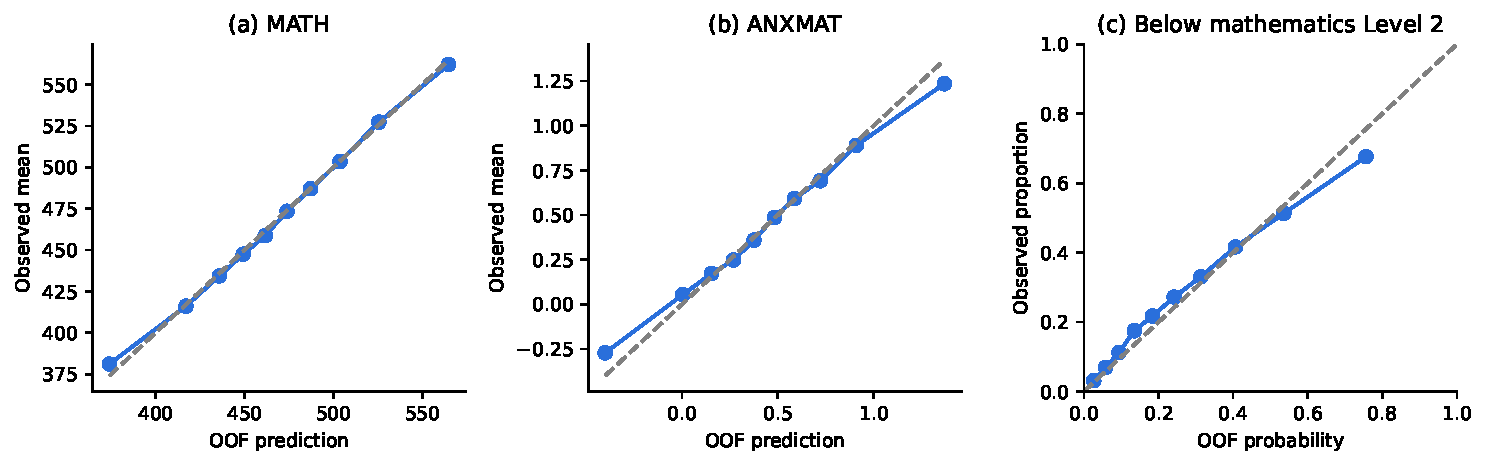
\includegraphics[width=\textwidth]{FigU_calibration.pdf}
\caption{Out-of-fold reliability, Viet Nam, PISA 2022: (a) mathematics regression ($n=6,068$, 178 schools); (b) anxiety regression ($n=5,934$, 178 schools); (c) separate classification of mathematics below Level 2, threshold 420.07 points \citep{oecd2023vol1}. Points are final-weighted means within predicted deciles; the dashed diagonal indicates perfect calibration. Mathematics panels average all ten plausible values. No confidence bands or significance tests are implied.}\label{fig:calibration}\end{figure}

The separate below-Level-2 classifiers have mean weighted Brier score 0.164, compared with 0.203 for each fold's training-prevalence baseline. Brier evaluates probabilities for this binary diagnostic, not the continuous regression. The predictions are retrospective associations using concurrent questionnaire data, not a validated prospective screening tool.

\begin{table}[H]\centering\scriptsize
\caption{Mathematics 2012--2022: link-error sensitivity in comparison systems}\label{tab:linkerror}
\begin{tabular}{@{}lrrrrr@{}}
\toprule
System & Difference & Sampling/PV SE & Link error & Total SE & 95\% interval\\
\midrule
HKG & -20.9 & 4.4 & 3.6 & 5.7 & [-32.0, -9.8]\\
IDN & -9.6 & 4.7 & 3.6 & 5.9 & [-21.1, 1.9]\\
JPN & -0.8 & 4.6 & 3.6 & 5.9 & [-12.3, 10.6]\\
KOR & -26.5 & 6.0 & 3.6 & 7.0 & [-40.1, -12.8]\\
MAC & 13.8 & 1.5 & 3.6 & 3.9 & [6.2, 21.4]\\
MYS & -11.8 & 4.0 & 3.6 & 5.4 & [-22.3, -1.3]\\
SGP & 1.2 & 1.8 & 3.6 & 4.0 & [-6.7, 9.1]\\
TAP & -12.7 & 5.0 & 3.6 & 6.2 & [-24.8, -0.7]\\
THA & -32.8 & 4.4 & 3.6 & 5.6 & [-43.9, -21.7]\\
VNM & -- & -- & -- & -- & --\\
\bottomrule
\end{tabular}
\par\smallskip\raggedright\footnotesize Student final weights; cycle means combine BRR sampling and plausible-value uncertainty. Total SE is $\sqrt{SE_{2012}^2+SE_{2022}^2+3.58^2}$, using the mathematics link error reported in NCES technical notes, Table 3 (sourced to OECD) \citep{nces2023technical}. This is a two-cycle difference, not an all-cycle trend model. Viet Nam is excluded because OECD does not establish a reliable link with its prior performance results \citep{oecd2023vnm}; adding generic link error would not repair that problem. The adjustment does not apply to questionnaire proportions or within-cycle regressions.
\end{table}
